\newpage
\section{Evaluation}
For the evaluation of the user experience, 14 users tested the tool.
After a week, test users completed a survey that contained questions about how understandable the information was
and how useable it was. Additionally, respondants could make their own comments.
\begin{figure}[ht]
   \centering
   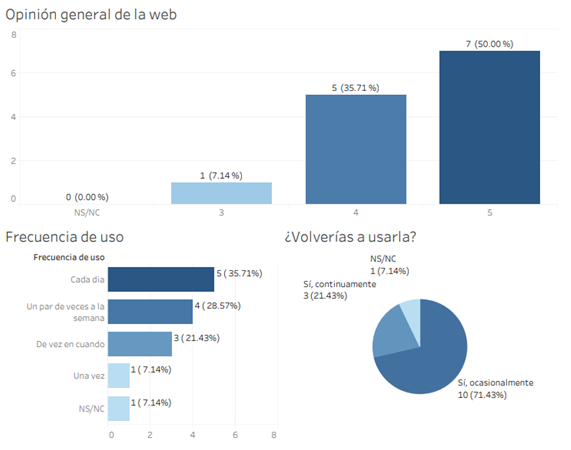
\includegraphics[width=12cm]{enqueteResults}
   \caption{Part of the user experience enquete results}
\end{figure}

Most of the respondents agreed that the functionality they liked the most, was to see the air quality index actually in the
map, and suggested increasing the number of zones.
92 \% of the respondents found the information useful and complete, and 71.43 \% answered that they also found it
understandable.
More than half of the respondents admit that they did not know the meaning of the air quality index, but after
using the tool, they now understand it.
Regarding their interest about air quality, half of them indicated that they had never sought information about it,
only two were previously well informed, and one of them marked the 'other' option and specified that using the application had aroused their interest.
In addition, four of them indicated that, thanks to the tool, they have now discovered they have a medical condition that is affected by air quality.

Among the test subjects, a greater awareness of pollution has been recognized, and they now show more interest in the
air quality in the city and its possible effects on their health.
